\documentclass[preprint]{sigplanconf}

% The following \documentclass options may be useful:
%
% 10pt          To set in 10-point type instead of 9-point.
% 11pt          To set in 11-point type instead of 9-point.
% authoryear    To obtain author/year citation style instead of numeric.

\usepackage{amsmath}
\usepackage{graphicx}

\begin{document}

\conferenceinfo{ICFP '13}{date, Boston} 
\copyrightyear{2013} 
\copyrightdata{[to be supplied]} 

\titlebanner{Red-Black Tree Deletion}        % These are ignored unless
\preprintfooter{Presents the missing method of Okasaki's red-black trees.}   % 'preprint' option specified.

\title{Deletion: The Curse of the Red-Black Tree}
\subtitle{Functional Pearl}

\authorinfo{Kimball Germane\and Matt Might}
           {University of Utah}
           %{Email2/3}

\maketitle

\begin{abstract}
Red-black trees were born in the imperative world and only adopted into the functional. Okasaki's exposition of the simplicity of a functional implementation actually felt more like a rebirth than mere adoption. With this regime shift came a shift in focus: the energy that would otherwise have been spent on pointer manipulation is now applied to establishing correctness with formal methods--a step forward, to be sure--but one wonders if there is a simple, obviously-correct, functional delete. Indeed there is.
\end{abstract}

\category{CR-number}{subcategory}{third-level}

\terms
red-black tree, delete, data structure

\keywords
red-black tree, delete, data structure

\section{Introduction}

When looking for a data structure to back a functional implementation of sets, red-black trees--a type of balanced binary search tree--are a natural choice. Common set operations, such as membership testing and persistent addition, map naturally to their native operations of search and insertion. And, speaking of maps, minor modifications can turn a set membership test into a map lookup operation and set addition into map extension. Used in this way, red-black trees are efficient, persistent, and still leave us wanting.

To see why, let's briefly review what makes red-black trees so special. A red-black tree is a binary tree in which each node is colored red or black, and which satisfies the local property that
\begin{enumerate}
\item every red node has two black children,
\end{enumerate}
and the global property that
\begin{enumerate}
\setcounter{enumi}{1}
\item every path from the root to a leaf\footnote{For our purposes, leaf nodes do not contain data and are always colored black.} node contains the same number of black nodes.
\end{enumerate}
These conditions guarantee that the longest path from root to leaf can be no more than twice the shortest (the only difference being individual red nodes interspersed along the way), and so the worst-case penalty for a tree search is a reasonable constant factor.

\section{Insertion}

Okasaki \cite{okasaki1999functional} made functional red-black trees accessible by presenting a clear method for element insertion by means of the recursive \texttt{insert} function and the \texttt{balance} helper function.

Using a bit of syntactic sugar on top of Racket, we can express the \texttt{insert} function with
\begin{verbatim}
(define (insert t v)
  (match t
    [(L) (R (L) v (L))]
    [(N c a x b)
     (switch-compare
       (v x)
       [< (balance (N c (insert a v) x b))]
       [= (N c a x b)]
       [> (balance (N c a x (insert b v)))])]))
\end{verbatim}
where \texttt{balance} yet remains undefined.

This definition of \texttt{insert} unilaterally colors each newly-added node red. If the parent of this new node is red, this action violates the local property. Okasaki persists in the face of this possibility, reasoning that it is easier to resolve a violation of the local property than the global one. This is done by the \texttt{balance} function which takes trees of the form
\begin{center}
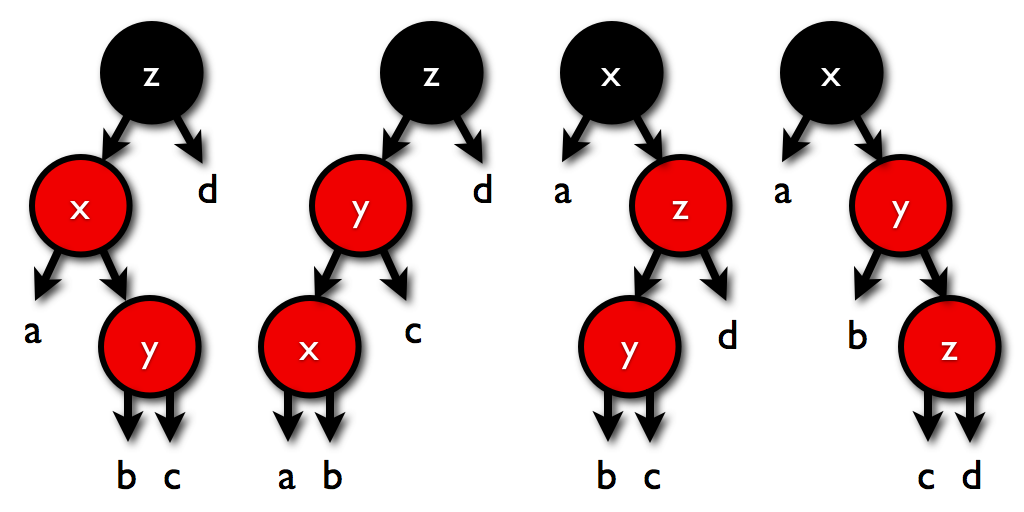
\includegraphics[scale=0.22]{four-cases.png}
\end{center}
and transforms them into
\begin{center}
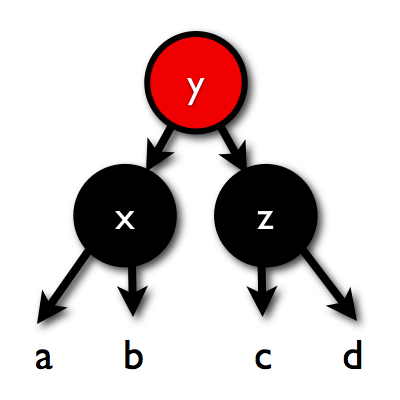
\includegraphics[scale=0.22]{four-cases-resolved.png}
\end{center}

We can reason about the effect this transformation has on the local property by considering the possible colorings of the root of each subtree $a$, $b$, $c$, and $d$. If the parent of this node is red, this node must be black and there are no restrictions on its placement in the reconstruction. If the parent is black, this node is possibly red, and the assignment of a red parent possibly introduces a red-red violation. The \texttt{balance} function is designed to resolve precisely this situation. We can verify this transformation preserves the global property by verifying that any possible introduction of this violation is subjected to \texttt{balance}.

Furthermore, we can reason locally about the effect this transformation has on the \emph{global} property by considering the number of black nodes this portion of the tree contributes to each path that travels through it. We can see that this transformation preserves the global property by verifying that the paths that reach the subtrees $a-d$ accumulate the same number of black nodes both before and after it occurs.

The purpose of this transformation is to resolve a violation of the local property, and while it does resolve one, it potentially introduces another further up the tree. We can treat this violation the same way and even with the same function; hence, the \texttt{balance} function is applied preventively at each level of the recursion which has the effect of working up the tree as the semantic stack unwinds. This transformation cannot possibly introduce a red-red violation at the root of the tree, being the child of no node, so the correctness of the entire process follows from a simple inductive argument.

Much of the simplicity of Okasaki's explanation comes from the simplicity of going from the diagrams to
\begin{verbatim}
(define/match balance
  [(or (B (R (R a x b) y c) z d)
       (B (R a x (R b y c)) z d)
       (B a x (R (R b y c) z d))
       (B a x (R b y (R c z d))))
   (R (B a x b) y (B c z d))]
  [t t])
\end{verbatim}

The final stop of Okasaki's insertion algorithm is to blacken the root of the tree, which is benign in all cases. This requires a small modification of \texttt{insert} to 
\begin{verbatim}
(define (insert t v)
  (define (ins t v)
    (match t
      [(L) (R (L) v (L))]
      [(N c a x b)
       (switch-compare
         (v x)
         [< (balance (N c (insert a v) x b))]
         [= (N c a x b)]
         [> (balance (N c a x (insert b v)))])]))
  (blacken (ins t v)))
\end{verbatim}
with a trivial definition of \texttt{blacken}.


%We can reason about this transformation purely locally by considering the number of black nodes this portion of the tree contributes to each path that travels through it.

%It is easy to see that this transformation brings this part of the tree in harmony with the local condition. We can reason that it preserves the global property by considering the number of black nodes this portion of the tree contributes to each path that touches it. Each of these paths a, b, c, and d passes through the single black node atop each case. Then the product of the transformation must be correct as each path inherits/accesses/utilizes one black node [in the target].

\section{Deletion}

Maybe move.

In addition to introducing a functional treatment of tree insertion, Okasaki succeeded in adding intuition to something generally considered to be intricate and error-prone. The net effect of his contribution is not code so short that it is easily memorizable but a concept so elegant and natural that, from it, the code is easily derivable--very befitting of its pearl namesake. As a result, the attitude of intricacy and proneness to error has shifted to tree deletion. While we grant that deletion seems to be more complex than insertion, we hope to show that it is only slightly so, and that, with the right intuition, it can enjoy the same status as insertion.

Deletion in unrestricted binary search trees is fairly straightforward. First, locate the node that contains the value to delete. If the node has no right subtree, replace it with its left subtree. If it has a right subtree, replace its value with the minimum value of its right subtree and remove that value from the right subtree.\footnote{An alternative is to distinguish left subtrees and use the maximum element. By considering right subtrees, we get a \texttt{min\_element} function for free, which is critical for priority queues.} Thus, deletion is recursive.

We can modify this approach to account for red-black properties and ultimately preserve them. We start by considering the configurations of a node with no right subtree.

The empty tree
\begin{center}
\includegraphics{empty.pdf}
\end{center}
remains unchanged after the removal of any element.

A red node with no left or right subtree
\begin{center}
\includegraphics{single-red.pdf}
\end{center}
becomes the empty tree.

A red node with a black-rooted left subtree
\begin{center}
\includegraphics{red-black-left-subtree.pdf}
\end{center}
violates the global property and cannot occur.

A black node with a red-rooted left subtree
\begin{center}
\includegraphics{black-red-left-subtree.pdf}
\end{center}
becomes the subtree itself, only black-rooted. The global invariant dictates that the left subtree is at most a single red node, so there is no chance that this introduces a violation.

Finally, a black node with no left or right subtree
\begin{center}
\includegraphics{single-black.pdf}
\end{center}
presents us with a challenge. The paths that end at one of its leaves accumulate two black nodes from this portion of the tree--one for the node itself and one for the leaf. If we were to treat this case the same as if the node were red, we would violate the global property. Repurposing some wisdom from Okasaki, perhaps we should attempt to preserve the global property at the expense of something more local. We do this by introducing a new node color, double-black, and a new leaf node, the double-black leaf.

For accounting purposes, a double-black node contributes two black nodes to any path that travels through it. Of course, we cannot let such a node persist, or we'll have no hope of maintaing optimal time complexity. We can attempt to discharge it by performing a tree rotation...

Much like insertion, we have to account for the possibility of a deletion operation introducing a double-black node from the start. Where the insertion operation balances the tree, attempting to resolve red-red violations, the deletion operation rotates the tree, attempting to discharge double-black nodes. Just as the insertion operation possibly passes unbalance up the tree, the deletion operation possibly passes a double-black node up the tree. Finally, both operations ``bottom out'' at the top of the tree, guaranteeing resolution.

The final step of Okasaki's algorithm unilaterally changes the root node to black. The red-black invariants, as we have formulated them, allow trees to have red roots in some cases, so our root-coloring policy is more conservative, only blackening if the red-black construction demands it.

When inserting an element, our final step is to blacken the root, but only if necessary. Dual to this, when deleting an element, our \emph{first} step is to redden the root, but only if possible. This gives us slack if the ascending rotations happen to make it to the root. (If we are unable to redden the tree without violating the local condition, then at least on of the children must itself be red which puts a red node sufficiently close to the action.)

The delete function first locates the given value in recursive fashion. If we reach a leaf node, the value was not present, and the tree is left unchanged. If it is found at the bottom and colored red, it is soundly removed. If it is colored black, we replace it with a double-black leaf. If we imagine that such a leaf counts for two black nodes, thin this action preserves the global property. Of course, the properties are simply to guarantee specific time complexities, and traversing this node costs no more than traversing any other. This node is a temporary marker to indicate the need for rotation, and will be discharged accordingly.

If the value is found enough away from the fringe, we replace it with the minimum value of its right child and remove the node that contained that. This strategy is convenient for two reasons: First, it allows us to provide or leverage a \emph{min} function, which is useful when implementing priority queues. Second, it allows us to only worry about removing nodes from the bottom of the tree.

We must consider the final case when the value resides in node not on the bottom of the tree, but with no right child. In this case, the global condition constrains the node to be black and its sole child to be red. To satisfy this case, we remove the black node and replace it with its child, colored black. In doing this, we face no danger in violating either constraint.

In the same way that we consider leaf nodes to be black, we consider double-black leaf nodes to be double black.

The presence of a double-black child node indicates the need for a rotation operation. In some cases, the rotation can discharge the double-black node, and no further rotations will be made. In others, the local structure of the tree prevents resolution in its scope, and the double-black node is pushed higher to be treated by another rotation occurring higher in the tree.

We might ask whether a double black node will reach the top before resolution. Such an occurrence would not be fatal since we could soundly demote it to a single-black node once at the root. This would require a minor intrusion of concerns into the \emph{blacken} function, but is fortunately unnecessary. [Recall that] the first step of the deletion algorithm is to redden the root if possible, and that, if it's not possible, the root must have a red child. This is sufficient to guarantee that a double-black node, if it reaches the top, can be discharged there by the natural flow of the algorithm; no exceptions need be made.

In doing so, he overcame one deficiency and exposed another: the delete operation. Multiple strategies have been developed to offer the delete operation, but each has its own weakness.

Suppose we have a basic implementation of a red-black tree in a language that supports variants and pattern matching. Following Okasaki \cite{okasaki1999functional}, such an implementation might look like this:

\begin{verbatim}
data Color = R | B
data Tree a = E | T Color (Tree a) a (Tree a)

type Set a = Tree a

empty :: Set a
empty = E

member :: Ord a => a -> Set a -> Bool
member x E = False
member x (T _ l y r) | x <  y = member x l
                     | x == y = True
                     | x >  y = member x r 

insert :: (Ord a) => a -> Set a -> Set a
insert x s = makeBlack (ins s)
  where ins E = T R E x E
        ins (T color l y r) | x <  y = balance color (ins l) y r
                            | x == y = T color a y b
                            | x >  y = balance color l y (ins r)
        makeBlack (T _ l y r) = T B l y r
\end{verbatim}
Once the need for balancing is properly motivated and intuition described, the [novelty,bulk,workhorse,?] of the algorithm lies in the \texttt{balance} operation. The punchline of Okasaki's exposition is this simple, elegant implementation.
\begin{verbatim}
balance B (T R (T R a x b) y c) z d
     || B (T R a x (T R b y c)) z d
     || B a x (T R (T R b y c) z d)
     || B a x (T R b y (T R c z d)) = T R (T B a x b) y (T B c z d)
balance color a x b = T color a x b
\end{verbatim}

Red-black trees have a local [more like recursive] invariant which induces a global property.

\section{Deletion}

To support this operation, he suggests the approach of marking nodes as deleted instead of removing them from the tree outright \cite[p. 50]{okasaki1996purely}. This approach trades a rebalancing operation at removal for a global tree rebuild at time indeterminate ( and preserves time complexity only by amortizing the cost). This approach has other disadvantages. First, it contaminates the implementation: every operation needs to be taught about the deletion field and how to handle nodes so marked [, and the global rebuild condition must be tracked]. [Show example if need content.] Second, retaining references to ``deleted'' node data prevents it from being garbage-collected. [Elaborate if need content.]

To support deletion using this strategy, we first introduce a flag in the datatype indicating whether the element should be considered present or not, and teach the operations on that data type about the flag.
\begin{verbatim}
data Color = R | B
data Tree a = E | T Color Bool (Tree a) a (Tree a)

type Set a = Tree a

empty :: Set a
empty = E

member :: Ord a => a -> Set a -> Bool
member x E = False
member x (T _ f l y r) | x <  y = member x l
                       | x == y = f
                       | x >  y = member x r 

insert :: (Ord a) => a -> Set a -> Set a
insert x s = makeBlack (ins s)
  where ins E = T R True E x E
        ins (T color flag a y b) | x <  y = balance color flag (ins a) y b
                                 | x == y = T color True a y b
                                 | x >  y = balance color flag a y (ins b)
        makeBlack (T _ f a y b) = T B flag a y b
\end{verbatim}
We omit the corresponding changes to \texttt{balance}. With that in place, a first pass at a \cite{delete} operation can be made:
\begin{verbatim}
delete :: Ord a -> a -> Set a -> Set a
delete x E = E
delete x (T color flag a y b) | x <  y = T color flag (delete x a) y b
                              | x == y = T color False a y b
                              | x >  y = T color flag a y (delete x b)
\end{verbatim}
The implementation is certainly correct, but it removes the time complexity guarantee that is worth the conceptual complexity. In order to preserve that, we introduce the necessary bookkeeping to trigger a global rebuild at the proper time.
\begin{verbatim}
data Color = R | B
data Tree a = E | T Color Bool Int Int (Tree a) a (Tree a)
...
\end{verbatim}
Once the need for balancing is properly motivated and intuition described, the [novelty,bulk,workhorse,?] of the algorithm lies in the \texttt{balance} operation. The punchline of Okasaki's exposition is this simple, elegant implementation.
\begin{verbatim}
balance B (T R (T R a x b) y c) z d
     || B (T R a x (T R b y c)) z d
     || B a x (T R (T R b y c) z d)
     || B a x (T R b y (T R c z d)) = T R (T B a x b) y (T B c z d)
balance color a x b = T color a x b
\end{verbatim}

%The appropriate choice of node type for a red-black tree allows it to be used for a variety of applications. (Yuck.) A singleton allows it to back mathematical sets with insert and member? operations. A pair allows it to implement dictionaries with set and lookup operations. etc. No choice of node can compensate for the lack of a remove operation.

%Removal of [Okasaki] nodes from trees can be accomplished by marking a node as deleted and deferring the actual removal to a batch removal performed when deleted nodes begin to outnumber the others. This operation gives even lower than amortized logarithmic time complexity and doesn't interfere with the complexity of other tree operations.

%What is the argument for a removal operation with immediate complexity of O(log n)?
%Okasaki's thesis, page 50 (as numbered), par. 3: this mentions the cost of marking the node as deleted, but doesn't factor it into the amortized cost, correct? If we have n nodes and "delete" n/2, that takes (n log n)/2 operations. The rebuild takes n operations. So the amortized complexity is [(n log n)/2 + n]/(n/2)=log n + 1/2, or log n. So, the complexity is the same, but there is a constant factor. What happens if we add and remove the element multiple times. The addition has an immediate complexity and so is taken care of. The deletion has an amortized complexity, but say each deleted node was added and deleted k times. Then more deletes are happening over which the n/2 cost is spread, so it's actually better.

%An immediate delete localizes the (conceptual /and/ time) complexity of the data structure. (Conceptually, because a counter needs to be kept in the other case, unless you want to incur an O(n) operation every time you want to delete.)

%A red-black tree must satisfy two invariants:



%The first invariant ensures that at most one red node can separate an otherwise parent and child. Coupled with the second invariant, we are guaranteed that the longest path from the root to an empty node is at most twice as long as the shortest path, with the difference made up by interspersed red nodes.

%There are x operations generally defined for red-black trees.

%Red-black trees are typically used as the backing store for finite subsets of 
%a totally-ordered set or finite maps with a totally-ordered domain.

%Emphasize that we would like to localize the complexity.

%If we mark nodes as deleted, every operation must know about deleted nodes.
%In order to add the delete operation [in this way], we must modify every 
%other operation.

%THIS IS BIG: real research is going to come from a question in the form of
%"prove or disprove". Being told something is true (or good) and asked to 
%justify it is going to lead to disintegrity.

%First, the implementation of a simple binary tree.

%data Tree a = Empty | Node a (Tree a) (Tree a)

%insert :: (Ord a) => Tree a -> a -> Tree a
%insert Empty x = Node x Empty Empty
%insert (Node y l r) x = | x < y     -> Node y (insert l x) r
%                        | otherwise -> Node y l (insert r x)

%count :: Tree a -> Int
%count Empty = 0
%count (Node \_ l r) = 1 + (count l) + (count r)

%member :: (Ord a) => Tree a -> a -> Boolean
%member Empty \_ = False
%member (Node y l r) x = x < y     -> member l x
%                        x > y     -> member r x
%                        otherwise -> True

%Deletion in a binary tree is fairly straightforward.

%delete :: (Ord a) => Tree a -> a -> Tree a
%delete Empty \_ = Empty
%delete (Node x l Empty) x = l
%delete (Node x Empty r) x = r
%delete (Node x l (Node
%delete (Node y l r) x = x < y     -> Node y (delete l x) r
%                        x > y     -> Node y l (delete r x)
%                        otherwise ->

%data Color = Red | Black
%data Tree a = Empty | Node Color a (Tree a) (Tree a)

%enforcing invariants with types leads to Byz

Red-black trees were born in the imperative world and only adopted into the functional. Okasaki's exposition of the simplicity of a functional implementation actually felt more like a rebirth than mere adoption. With this regime shift came a shift in focus: the energy that would otherwise have been spent on pointer manipulation is now applied to establishing correctness with formal methods--a step forward, to be sure--but one wonders if there is a simple, obviously-correct, functional delete. Indeed there is.




Where imperative programmers devote their energies to pointer manipulation








Suppose the value we wish to delete happens to reside in a node at the bottom of the tree. There are two possibilites:

%\includegraphics[scale=0.20]{red-black-slides-008.png}

The delicate thing here is that we need to maintain the invariant that every path from the root of the tree to the bottom has the same number of black nodes. In the case that our value resides in a red node, we can intuitively see that replacing that entire subtree with a black leaf will preserve the invariant. A conceptual viewpoint that will serve us well is that the leaves donated their ``blackness'' to the parent, preserving the invariant. By applying the same idea to the second case, we must decide what happens when the ``blackness'' is propagated upward to a black node. As a conceptual convenience, we can temporarily assign the node a color of double black. This means that when counting the number of black nodes in a path which contains this node, we count this node twice. Of course, this is strictly for accounting purposes, and the node of course has the same computational cost to traverse as any other node. We will simply use this new color to account for bubbling which needs to travel up the tree.

Now we can consider the cases that the node is not at the end of the tree. First, consider the case where the node in question has only one child subtree. In order for this occur, the node would have to be black with a red child. (And we can say even more about this child: it has no children of its own, else the tree would stray from the path invariant.) The child becomes the parent and is made black. [Can we motivate this with the color arithmetic?]

learn the algorithm and then think about it.

\section{Conclusion}
It is true that genuine deletion is complex, but its complexity is fairly localized. Aside from the \texttt{delete} function proper, it requires the extension of the \texttt{Color} datatype to support two more atomic variants and a few helper functions to support color arithmetic. [It's a small price to pay.] In exchange, we receive O(log n) direct time complexity without any additional constant factor above the original implementation.



\appendix
\section{Appendix Title}

This is the text of the appendix, if you need one.

\acks

Acknowledgments, if needed.

% We recommend abbrvnat bibliography style.

\bibliographystyle{abbrvnat}
\bibliography{red-black-pearl}

% The bibliography should be embedded for final submission.

\begin{thebibliography}{}
\softraggedright

\bibitem[Smith et~al.(2009)Smith, Jones]{smith02}
P. Q. Smith, and X. Y. Jones. ...reference text...

\end{thebibliography}

\end{document}







